\documentclass{beamer}
\usepackage[utf8]{inputenc}
\usepackage{microtype}
\usepackage{default}

\usetheme{simple}
\usepackage[french]{babel}
\usepackage{fontspec}
\usepackage{graphicx}
\setmainfont{Fira Sans}
\setmonofont{Fira Code}
\usepackage{listings}
\usepackage{default}
\title{Outils spatiaux pour partitions interactives}
\author{Jean-Michaël Celerier\\ Myriam Desainte-Catherine\\ Jean-Michel Couturier}
\date{1er avril 2016}

\begin{document}
\begin{frame}
    \centering
    \maketitle
\end{frame}

\section{Problématique}
\begin{frame}
    \frametitle{Problématique}
    \centering\Large
    Mais d'abord, qu'est-ce qu'un espace ?~\\
    \vspace{2cm}
    $\rightarrow$ Un ensemble de dimensions bornées continues.
\end{frame}

\begin{frame}
    \frametitle{Problématique}
    \Large
    \begin{itemize}
        \item Définir des scénarios interactifs contenant des éléments spatiaux.
        \item Gérer des comportements multidimensionnels dans le temps.
        \item Problématique de l'UI d'écriture.
    \end{itemize}
    
    Objectif : 
    
    \begin{itemize}
        \item Décrire des interactions à plus d'une dimension de manière intégrée.
        \item Exemple : muséographie, contrôle de robots, jeux vidéos, musique spatialisée, \dots
    \end{itemize}
    
\end{frame}

\section{Approche}
\begin{frame}
    \frametitle{Approche}
    \Large
    \begin{itemize}
        \item Approche déclarative.
        \item Généralisation puis réduction : 
        \item Implémentation dans cas générique : forme cartésienne.
        \item Implémentations optimisées dans cas courants (OO). 
        \item Alternative : Constructive Solid Geometry.
    \end{itemize}
\end{frame}

%TODO montrer l'équation d'un cercle, mais aussi dans un espace

\begin{frame}
    \frametitle{Définition (1)}\Large
    \begin{itemize}
        \item On crée d'abord un espace : nombre de dimensions, bornes, granularité.
    \end{itemize}
    
    Ex. : 
    \begin{itemize}
        \item $x \in [-100; 100]$
        \item $y \in [0; 50]$
        \item Granularité : 5.
    \end{itemize}
\end{frame}

\begin{frame}[fragile]
    \frametitle{Définition (2)}\Large
    \begin{itemize}
        \item On définit des zones en donnant un ensemble d'équations cartésiennes qui les définissent.
        \item On sépare les variables en deux groupes : variables d'espace et paramètres.
        \item Transformations : échelle, rotation, translation.
        \item Fonctions autorisées : admissibles dans solutions en forme close ($\sin x, \cosh x, \ln x, \sqrt x, \dots)$. Pas d'$\int$.
        \item Paramètres des zones : peuvent être des constantes ou bien des adresses OSC.
    \end{itemize}
    
\end{frame}

\begin{frame}[fragile]
    \frametitle{Définition (2)}\Large
    Ex. : 
    
    \begin{lstlisting}[columns=fullflexible]
    u <= 0 ; (u - x0)^2 + (v - y0)^2 <= r0^2     
    \end{lstlisting}
    \begin{itemize}
        \item $u \leftarrow x$
        \item $v \leftarrow y$
        \item $x0 \leftarrow \mathtt{foo:/bar}$
        \item $r0 \leftarrow \mathtt{parent:/t}$
        \item $y0 \leftarrow 5$
    \end{itemize}
\end{frame}

\begin{frame}
    \frametitle{Définition (3)}\Large
    \begin{itemize}
        \item On définit des calculs et relations qui vont être évaluées entre zones.
        \item Actuellement : collision, distance (des barycentres). 
        \item À terme : pouvoir là aussi spécifier des formules.
        %TODO a1.x, a2.r ?
        %TODO METTRE  SCHEMA : passage 
    \end{itemize}
    ~\\
    Sémantique d'exécution : 
    \begin{itemize}
        \item On suit celle d'i-score : au tick.
        \item Utilisation récursive des résultats : décalage d'un tick.
    \end{itemize}
\end{frame}

    
    % TODO schéma contenu d'un tick : -> réception OSC, application aux zones, réalisation des calculs, écriture OSC

\begin{frame}
    \frametitle{Visualisation}
    \Large
    \begin{itemize}
        \item Actuellement, seulement 2D.
        \item Passage à la 3D : VTK? Qt3D?
        Pour zones génériques : triangulation (Delaunay).
        \item Passage en $n$ dim : par restriction à des sous espaces.
        \item À faire sur GPU pour cas général.
    \end{itemize}
\end{frame}


\begin{frame}
    \frametitle{Automations 3D}\Large
    \begin{itemize}
        \item Standard : équation paramétrique. Comme IanniX, OpenMusic...
        \item Courbe : parcourue dans son intégralité durant une contrainte temporelle.
    \end{itemize}
    \begin{figure}
        \centering
        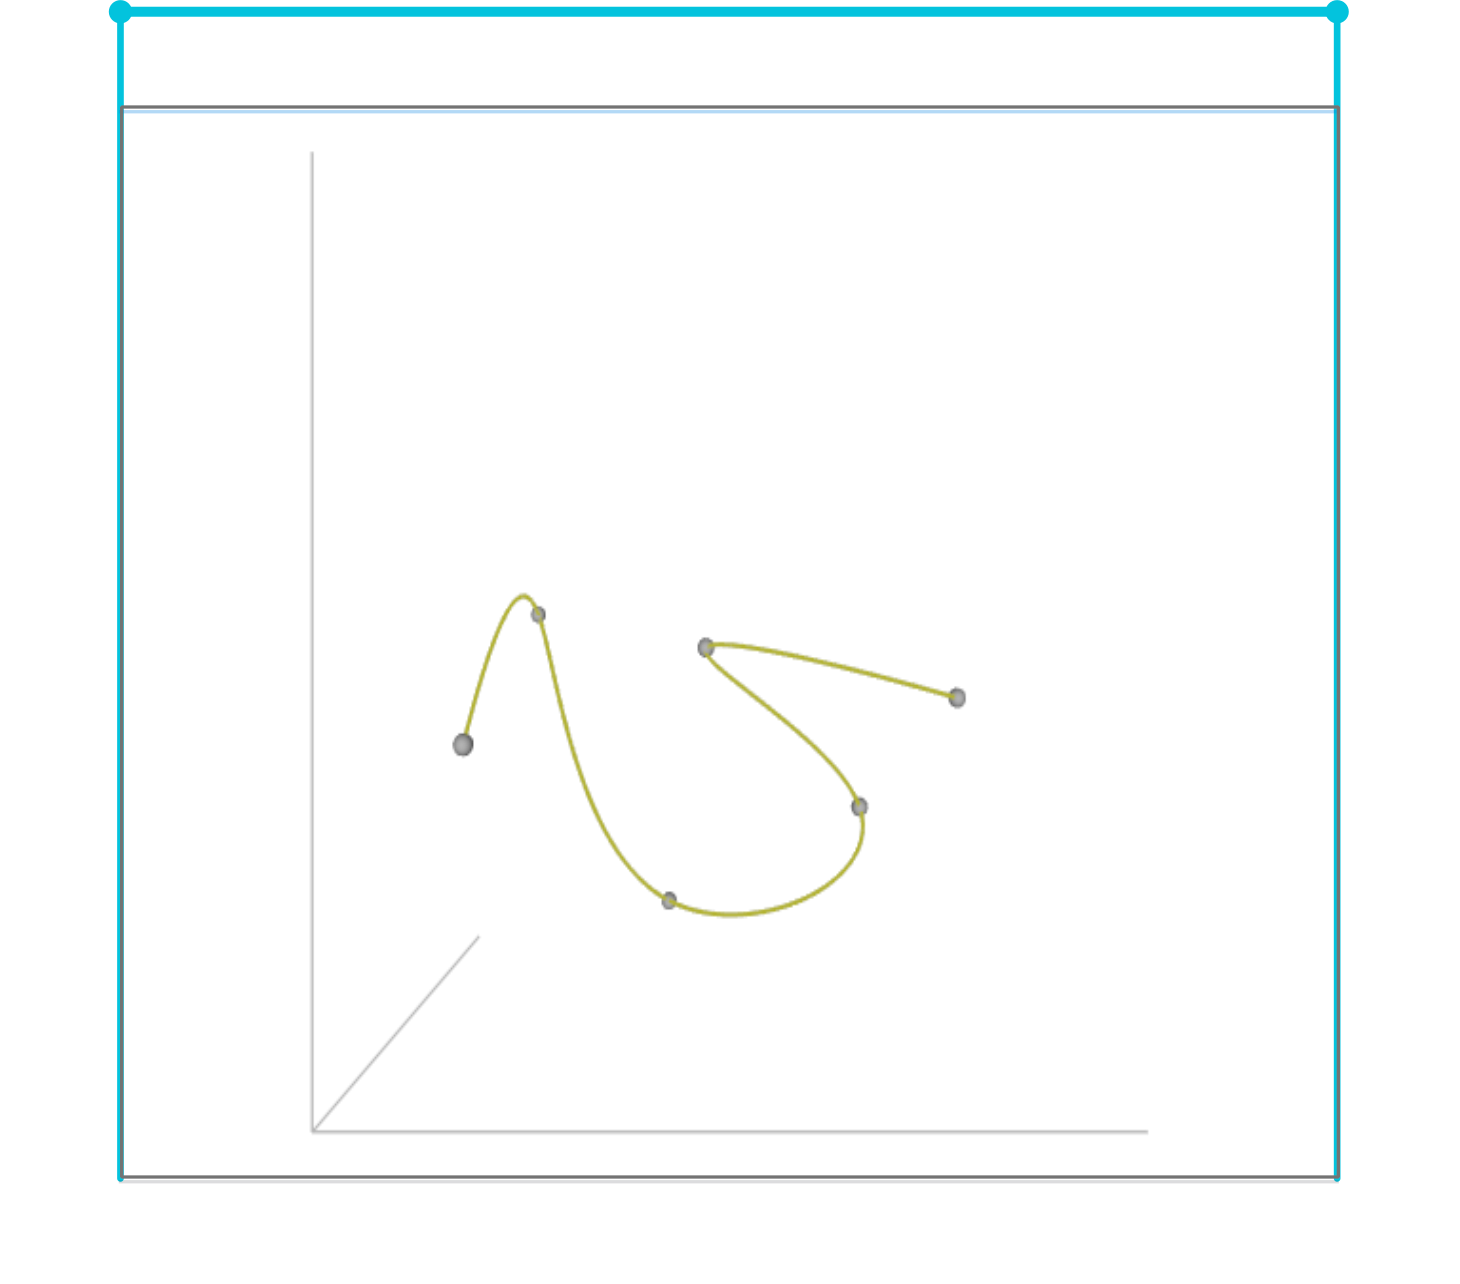
\includegraphics[scale=0.5]{images/autom3d.png}
    \end{figure}
\end{frame}

\begin{frame}
    \centering\huge
    Démonstration
\end{frame}

\section{Conclusion}

\begin{frame}
    \frametitle{Conclusion}
    \Large
    \begin{itemize}
        \item Présentation d'un modèle de définition d'objets spatiaux dans i-score.
        \item Géométries dynamiques.
        \item Problème : représentation disjointe d'un seul espace ? 
        \item Problème : représentation plus propre des ouverts ?
    \end{itemize}
\end{frame}
\begin{frame}
    \frametitle{Perspectives}
    \Large
    \begin{itemize}
        \item Écriture de scénarios spatiaux contraints : analogue d'i-score dans plus que 1D.
        \item Généraliser les deux en une méthode permettant d'étendre la notion de scénario interactif à des flux multi-dimensionnels.
        \item Actuellement, c'est fait... à la main dans i-score.
        \item Notion d'abstraction dans i-score : patch ?
        \item Compiler à la volée pour exec. plus rapide ? (Actuellement : \texttt{vtkFunctionParser}).
    \end{itemize}
\end{frame}


\begin{frame}
    \large{}
    \centering
    Merci de votre attention !~\\
    
    \Huge{}~\\
    Questions
\end{frame}

\end{document}
